\documentclass[a4paper,11pt,fleqn]{article}%fleqn pour aligner les equations à gauche
\usepackage{../../Styles/Cours}


\newcommand{\chnum}{Chapitre 17}
\newcommand{\chtitle}{Images et Couleurs}
\newcommand{\dtype}{Cours}

\begin{document}
	\maketitle

    \section{L'obtention des couleurs}
    Les procédés de synthèse additive et soustractives reposent sur la structure de l'\oe il humain. Celui-co perçoit les couleurs grâce à des récepteurs appelés cônes. Il en existe de trois types, chacun étant sensible à une longueur d'onde particulière de la lumière.
        \subsection{La synthède additive}
        \begin{minipage}{.7\linewidth}
            La superposition de trois \emph{lumières} colorées permet d'obtenir une infinité d'autres couleurs. À partir des trois couleurs primaires :  le bleu, le rouge et le vert, il est donc possible de produire des couleurs secondaires par superposition : le cyan, le jaune et le magenta.\\
            La superposition des trois couleurs peimaires donnant du blanc.
        \end{minipage}
        \begin{minipage}{.28\linewidth}
           \centering  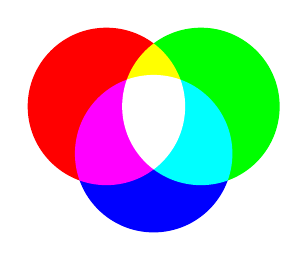
\begin{tikzpicture}
            \fill(0,0)[red,blend mode = screen] circle(1);
            \fill(1.2,0)[green,blend mode = screen] circle(1);
            \fill(.6,-.6)[blue,blend mode = screen] circle(1);
            \end{tikzpicture}
        \end{minipage}

        \subsection{La synthèse soustractive}
        \begin{minipage}{.7\linewidth}
            La superposition de \emph{pigments} colorés permet par synthèse soustractive, d'obtenir plusieurs couleurs. En partant des trois couleurs secondaires et en les superposant, on obtient les couleurs primaires.\\
            La superposition des trois couleurs secondaires donnant du noir.
        \end{minipage}
        \begin{minipage}{.28\linewidth}
            \centering  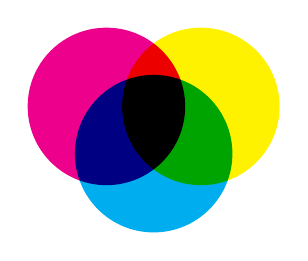
\begin{tikzpicture}
            \fill(0,0)[magenta,blend mode = multiply] circle(1);
            \fill(1.2,0)[yellow,blend mode = multiply] circle(1);
            \fill(.6,-.6)[cyan,blend mode = multiply] circle(1);
            \end{tikzpicture}
        \end{minipage}
    \section{La couleur des objets}
        \subsection{Interaction entre la lumière et l'objet}
        \begin{minipage}{.6\linewidth}
            Selon la nature et les caractéristiques physiques des objets, l'intéraction qu'ils auront avec la lumière incidente ne sera pas la même.\\
            Lorsqu'un objet reçoit  une lumière incidente, il peut :
            \begin{itemize}
                \item la transmettre :  l'objet est donc traversé par cette lumière (ex : solutions colorées)
                \item l'absorber : l'objet absorbe la lumière
                \item la diffuser : l'objet renvoie la lumière dans toutes les directions.
            \end{itemize}
            Dans al majorité des cas les trois phénomènes se produisent en même temps : en effet une partie de la lumière est absorbée par l'objet et une autre peut être transmise.\\
            Un objet coloré absorbe sa couleur complémentaire.
        \end{minipage}
        \begin{minipage}{.38\linewidth}
            \centering
            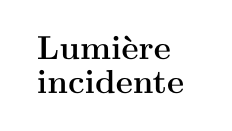
\begin{tikzpicture}
                \draw(0,5) node[text width = 2cm]{\centering \large \textbf{Lumière incidente}};
                
            \end{tikzpicture}
            
        \end{minipage}
\end{document}